\documentclass{standalone}
\usepackage{tikz}

\usepackage{tikzducks}

\begin{document}
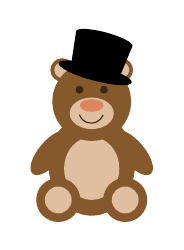
\begin{tikzpicture}
%  mitte: x=0.925

% Body %%%%%%%%%%%%%%%%%%%%%%%%%%%%%%%%%%%%%%%%%%%%%%%%%%%%%%%%%%%%%%%
\fill[brown!70!black] (0.925,0.75) ellipse (0.55 and 0.65); 
\fill[brown!50!white] (0.925,0.7) ellipse (0.35 and 0.4); 

% Feet %%%%%%%%%%%%%%%%%%%%%%%%%%%%%%%%%%%%%%%%%%%%%%%%%%%%%%%%%%%%%%%
\fill[brown!70!black] (1.35,0.3) circle (0.28); 
\fill[brown!70!black] (0.50,0.3) circle (0.28);
\fill[brown!50!white] (1.35,0.3) circle (0.17); 
\fill[brown!50!white] (0.50,0.3) circle (0.17);

% Ears %%%%%%%%%%%%%%%%%%%%%%%%%%%%%%%%%%%%%%%%%%%%%%%%%%%%%%%%%%%%%%%
\fill[brown!70!black] (1.30,1.95) circle (0.15);
\fill[brown!70!black] (0.55,1.95) circle (0.15);
\fill[brown!50!white] (1.30,1.95) circle (0.1);
\fill[brown!50!white] (0.55,1.95) circle (0.1);

% Head %%%%%%%%%%%%%%%%%%%%%%%%%%%%%%%%%%%%%%%%%%%%%%%%%%%%%%%%%%%%%%%
\fill[brown!70!black] (0.925,1.55) circle (0.5); 

% Muzzle %%%%%%%%%%%%%%%%%%%%%%%%%%%%%%%%%%%%%%%%%%%%%%%%%%%%%%%%%%%%%
\fill[brown!50!white] (0.925,1.4) ellipse (0.28 and 0.2); 
\fill[brown!70!white!80!red] (0.925,1.5) ellipse (0.15 and 0.08); 

% Eyes %%%%%%%%%%%%%%%%%%%%%%%%%%%%%%%%%%%%%%%%%%%%%%%%%%%%%%%%%%%%%%%
\fill[brown!30!black] (0.77,1.7) circle (0.05); 
\fill[brown!30!black] (1.08,1.7) circle (0.05); 

% Mouth %%%%%%%%%%%%%%%%%%%%%%%%%%%%%%%%%%%%%%%%%%%%%%%%%%%%%%%%%%%%%%
\draw[brown!30!black] (1.07,1.38) arc [start angle=-20, end angle=-160, radius=0.16];

% Arms %%%%%%%%%%%%%%%%%%%%%%%%%%%%%%%%%%%%%%%%%%%%%%%%%%%%%%%%%%%%%%%
\fill[brown!70!black,rotate around={-50:(1.45,0.9)}] (1.45,0.9) ellipse (0.35 and 0.15);
\fill[brown!70!black,rotate around={50:(0.4,0.9)}] (0.4,0.9) ellipse (0.35 and 0.15);

\duck[invisible,tophat]

\end{tikzpicture}
\end{document}